%!TEX root = /Users/manunavjeevan/Desktop/Research/Moment Inequality Methods/Annotated Literature Review/inequalityLitReview.tex

\newpage
\section{Set Identification in Models with Multiple Equilibria; \textit{\small Alfred Galichon, Marc Henry (ReStud, 2011)}}\label{sec:GH-2011}

\citet{GH-2011} proposes a computationally feasible way of deriving the identified features of a model with multiple equilibria in pure or mixed strategies. It can be found from the ReStud website \href{https://academic.oup.com/restud/article/78/4/1264/1593470}{here}.

\subsection{Introduction}

Empirical study of game theoretic models generally complicated by the presence of multiple equilibria. The existence of multiple equilibria generally leads to a failure of identification of the structural parameters governing the model.
\begin{itemize}
	\item Berry and Tamer (2006) and Ackerberg et al. (2007) give an account of the various ways this issue is approached in the literature.
	\item Andrews, Berry, and Jia (2003),  Ciliberto and Tamer (2009) consider some partial identification approach. Identification approach is not sharp.
\end{itemize}
Paper proposes a computationally feasible way of recovering the identified. Note a generalized likelihood implied by a model with multiple equilibria can be represented by a non-additive set function called a \textit{Choquet Capacity}.	Give a formal definition of an equilibrium selection mechanism and call such a mechanism compatible with the data if the likelihood of the model augmented with such a mechanism is equal to the probabilities observed in the data. THe identified feature of the model is then the set of parameter values s.t there exists an equilibrium selection mechanism compatible with the data.

The computational burden remains high in situations with a large number of observable outcomes since the number of inequalities to be checked is equal to the number of subsets of the set of observable outcomes.

\subsection{Identified Features of Models with Multiple Equilibria}
First go over framework and general results in the case where only equilibria in pure strategies are considered. Section 1.2 specializes and illustrates them on leading examples of participation games.

\subsubsection{Identified Parameter Sets in General Models with Multiple Equilibria}

General framework is that of Jovanovic (1989). Applies to the empirical analysis of normal form games, where only equilibra in pure strategies are considered. Consider three types of economic variables.
\begin{itemize}
	\item Outcome variables, $Y$
	\item Exogenous explanatory variables $X$
	\item Random shocks (or latent variables) $\epsilon$
\end{itemize}
Outcome variables and latent variables are assumed to belong to complete and separable metric spaces. Economic model consists of a set of restrictions on the joint behavior of the variables listed above. Restrictions may be induced by assumptions of rational agents, and they generally depend on a set of unknown structural parameters, $\theta$.

Without loss of generality, model may be formalized as a measurable correspondence (defined below) between the latent variables $\epsilon$ and the outcome variables $Y$, indexed by the exogenous variables $X$ and the vector of parameters $\theta$. This correspondence is called $G$ and write
$Y\in G(\epsilon | X;\theta)$ to indicate admissible values of $Y$ given $\epsilon, X, \theta$. The econometrician is assumed to have access to a sample of i.i.d vectors $(Y,X)$ and the problem that is considered is estimating the vector of parameters $\theta$. The latent variables $\epsilon$ is supposed to be distributed according to a parametric distribution $\nu(\cdot|X;\theta)$. Assumptions are collected below:
\newpage
\begin{assumption}
	\label{assm:GH-1}
	An independent and identically distributed sample of copies of the random vector $(Y,X)$ is available. The observable outcomes $Y$ conditionally distributed according to the probability distribution $P(\cdot|X)$ on $\calY$, a Polish space\footnote{A Polish space is a complete and separable metric space. A complete metric space is one where every Cauchy sequence converges to a point in the space and a separable metric space is one with a countable, dense, subset. A Cauchy sequence, $(a_n)_{n\in \SN}$ is one such that for every $\epsilon > 0, \exists N_\epsilon \in \mathbb{N}$ s.t $\forall m,n \geq N_\epsilon, d(a_m, a_n) < \epsilon$. Completeness ensures that the space is ``rich enough.'' For example, the reals are complete but the rationals are not.}
	endowed with its Borel $\sigma$-algebra of subsets $\calB$ are related to the unobservable variables $\epsilon$ according to the model $Y\in G(\epsilon| X;\theta)$. Here, $\theta$ belongs to an open subset $\Theta$ of $\SR^{d_\theta}$, $\epsilon$ is distributed according to the probability measure $\nu(\cdot|X;\theta)$ on $\calU$\footnote{Also a Polish space},
	and $G$ is a measurable correspondence\footnote{A measurable correspondence is such that for all open subsets $A \subseteq \calY$, $G^{-1}(A|X;\theta) := \{\epsilon\in\calU: G(\epsilon|X;\theta) \cap A \neq 0\}$ is measurable. A note: technically $A$ should be measurable, but since we are dealing with Borel $\sigma$-algebra's this is an equivalent definition. A measurable correspondence is also called a random correspondence or a random set.}
	for almost all $X$ and for all $\theta \in \Theta$. Finally, the variables $(Y,X,\epsilon)$ are defined on the same underlying probability space $(\Omega, \calF, \mathbb{P})$.
\end{assumption}

\begin{example}
	\label{ex:GH-1}
	To illustrate, consider a simple game proposed by Jovanovic (1989). Consider two firms with profit functions $\Pi_1(Y_1, Y_2, \epsilon_1, \epsilon_2;\theta)= (\theta Y_2 - \epsilon_2)Y_1$ and $\Pi_2(Y_1, Y_2, \epsilon, \epsilon_2; \theta) = (\theta Y_1 - \epsilon_1)Y_2$ where $Y_i \in \{0,1\}$ is firm $i$'s action and $\epsilon = (\epsilon_1, \epsilon_2)$ are exogenous cots. The firms know their costs, the analyst only knows that $\epsilon$ is uniformly distributed on $[0,1]^2$ and that the structural parameter $\theta$ is in $(0,1]$. There are two pure strategy Nash equilibria. The first is $Y_1 = Y_2 = 0$ for all $\epsilon \in [0,1]^2$.  The second is $Y_1 = Y_2 = 1$ for all $\epsilon \in [0,\theta]^2$ and $Y_1 = Y_2 = 0$ otherwise. Hence the model is described be the correspondence $G(\epsilon; \theta) = \{(0,0),(1,1)\}$ for all $\epsilon \in [0,\theta]^2$ and $G(\epsilon;\theta) = \{0,0\}$ otherwise.
\end{example}

To conduct inference on the parameter vector $\theta$, one first needs to determine the identified features of the model. Since $G$ may be multi-valued due to the presence of multiple equilibria, the outcomes may not be uniquely determined by the latent variable. In such cases, the generalized likelihood of an outcome falling in the subset $A$ of $\calY$ predicted by the model is $\calL(A|X;\theta) = \nu(G^{-1}(A|X;\theta)|X;\theta)$. Because of multiple equilibria, this generalized likelihood may sum to more than one, as we may have $A\cap B = \emptyset$ and yet $G^{-1}(A | X;\theta) \cap G^{-1}(B|X;\theta) \neq 0$\footnote{Intuition: $G^{-1}(y|X;\theta)$ gives the set of $\epsilon$ values that could have generated the $y$ value (observed outcome) conditional on $X$ and $\theta$ and one epsilon can generate two different $y$ values because of multiple equilibria.} so that for these sets $A,B$ such that $A \cap B = \emptyset$, $\calL(A\cup B | X;\theta) < L(A|X;\theta) + L(B|X;\theta)$. The set function $A\mapsto \calL(A|X;\theta) = \nu(G^{-1}(A|X;\theta)|X;\theta)$ is generally not additive and is called a \textit{Choquet capacity}\footnote{See Choquet, 1954. Choquet capacity also used as a generalized probability in some behavioral decision making theory.}. This non-additivity of the model likelihood is well documented.

\begin{definition}[Choquet capacity]
	\label{def:GH-1}
	A Choquet capacity $\calL$ on a finite set $\calY$ is a set function $\calL: A\subset\calY\mapsto[0,1]$ which is
	\begin{itemize}
		\item normalized, i.e $\calL(\emptyset) = 0$ and $\calL(\calY) = 1$
		\item monotone, i,e $\calL(A) \leq \calL(B)$, for any $A\subset B\subset \calY$
	\end{itemize}
\end{definition}

This is like a probability measure but without additivity. In the example above, $\nu(\cdot| X;\theta)$ is the uniform distribution on $[0,1]^2$ and the Choquet capacity $\nu(G^{-1})$ gives value $\nu(G^{-1}(\{0,0\})) = \nu([0,1]^2) = 1$. and $\nu(G^{-1}\{1,1\}) = \nu([0,\theta]^2)= \theta^2$ to the set $\{(1,1)\}$. Hence it is immediately apparent that the Choquet capacity of $\nu(G^{-1})$ is nonadditive.

As discussed in Jovanovic (1989) and Berry and Tamer (2006), the model with multiple equilibria can be completed with an equilibrium selection mechanism. Define an equilibrium selection mechanism as a conditional distribution $\pi_{Y|\epsilon, X;\theta}$ over equilibrium outcomes $Y$ in the regions of multiplicity. By construction, an equilibrium selection mechanism is allowed to depend on the latent variables $\epsilon$ even after conditioning on $X$.

\begin{definition}[Equilibrium selection mechanism]
	\label{def:GH-2}
	An equilibrium selection mechanism is a conditional probability $\pi(\cdot|\epsilon, X;\theta)$ for $Y$ conditional on $\epsilon$ and $X$ such that the selected value of the outcome variable is actually an equilibrium. Formally $\pi(\cdot|\epsilon, X,\theta)$ has support contained in $G(\epsilon|X;\theta)$.
\end{definition}

Crucial to this is the fact that $\pi$ is a \textit{probability measure}. It should ``smooth out'' the non-additivity of $\nu(G^{-1})$.

\emph{The identified feature of the model is the smallest set of parameters that cannot be rejected by the data}. Hence, it is the set of parameters for which one can find an equilibrium selection mechanism that completes the model and equates probabilities of outcomes predicted by the model with the probabilities obtained from the data.\footnote{Is this somehow restrictive? I guess not, since we've placed no assumption on the selection mechanism.}

\begin{definition}[Compatible equilibrium selection mechanism]
	\label{def:GH-3}
	The equilibrium selection mechanism $\pi(\cdot|\epsilon, X;\theta)$ is compatible with the data if the probabilities observed in the data are equal to the probabilities predicted by the equilibrium selection mechanism. More formally, if for all measurable subsets $A$ of $\calY$
	\[P(A|X) = \int_\calU \pi(A|\epsilon, X,\theta) \nu(d\epsilon |X;\theta)\]
\end{definition}
\begin{definition}[Identified Set]
	\label{def:GH-4}
	The identified set (or the \emph{sharp} identified set) is the set $\theta_I \subseteq\Theta$ such that, $\forall \theta \in \theta_I$, there exists an equilibrium selection mechanism compatible with the data.
\end{definition}

Above definition is not operational, in the sense that it does not allow for the computation of the identified set based on the knowledge of the probabilities in the data, because $\pi$ is an infinite dimensional nuisance parameter. Now set out to show how to reduce the dimensionality of the problem. Equivalent formulation of the identified set relates to the \emph{core} of the Choquet capacity.
\begin{definition}[Core of a Choquet capacity]
	\label{def:GH-5}
	The \emph{core} of a Choquet capacity $\calL$ on $\calY$ is the collection of probability distributions $Q$ on $\calY$ such that for all $A\subset \calY$, $Q(A) \leq \calL(A)$.
	\footnote{Equivalently, if we consider the random set $\calL$ as a map from $(\Omega, \calF, \mathbb{P}) \rightarrow 2^\calY$, we can say a random variable $\gamma:\Omega \rightarrow \calY$ is in the core of $\calL$ if $\gamma(\omega) \in \calL(\omega), \forall \omega \in \Omega.$ The random variable $\gamma$ induces a distribution on $\calY$ that has the above property, and every distribution on $\calY$ with the above property should be induced by a random variable with this property.}
\end{definition}
In cooperative game theory, a Choquet capacity on a set $\calY$ is interpreted as a game, where $\calY$ is the set of players and $\calL$ is the utility value or worth of a coalition $A\subseteq\calY$ and the core of the game $\calL$ is the collection of allocations that cannot be improved upon by any coalition of players.

In Example~\ref{ex:GH-1}, the core of the Choquet capacity $\nu G^{-1}$ is the set of probabilities $P$ for the observed outcomes $(0,0)$ and $(1,1)$ such that $P(\{(0,0)\}) \leq \nu G^{-1}(\{(0,0\}) = \nu([0,1]^2) =1$ and $P(\{(1,1)\}) \leq \nu G^{-1}(\{(1,1)\}) = \nu([0,\theta]^2) = \theta^2$.

Next result shows the equivalence between the existence of a compatible eqm. selection mechanism and the fact that the true distribution of the data belongs to the core of the Choquet capacity that characterizes the generalized likelihood predicted by the model.

\begin{theorem}
	\label{thm:GH-1}
	The identified set $\Theta_I$ is the set of parameters such that the true distribution of the observable variables lies in the core of the generalized likelihood predicted by the model.
	\[\Theta_I = \left\{\theta \in \Theta: \forall A \in \calB, P(A|X) \leq \calL(A|X;\theta); X-\text{a.s}\right\}\]
\end{theorem}

A later theorem generalizes this to the case of mixed strategy eqm. In the example above, the identified set is the set of values for $\theta$ such that $0 \leq \mathbb{P}((Y_1,Y_2)) \leq \theta^2$.

The first thing to note from this theorem is that the problem of computing the identified set has been transformed into a finite-dimensional problem in the case where $\calY$ is a finite set. Indeed, in this case, the problem of computing the identified set is reduced to the problem of checking a finite number of inequalities.

However, in cases where the cardinality of $\calY$ is large, then the number of inequalities to be checked is $2^{|\calY|} - 2$ and the computational burden is only partially lifted. The rest of the paper is based on the characterization of Theorem~\ref{thm:GH-1}.
\subsubsection{Some illustrative examples}

Examples are given in this section of Market Entry, Family Bargaining etc. For the most part, they resemble the market entry example given above in Section~\ref{sec:CCK-2019}.

\paragraph{Family Bargaining}

Go over this game since it is later considered in the optimal transport section. Consider a simplified version of the bargaining model of decision regarding the long-term care of an elderly parent for a family with two children. The issue is which child will care for the parent when the parent ages or whether the parent is moved to a nursing home. The payoff to family member $i, i = 1,2$ is represented by the sum of three terms.

The first term, $V_{ij}$ represents the value to child $i$ of care option $j$, where $j > 0$ means child $j$ becomes the primary care giver, and $j= 0$ means the parent is moved to a nursing home. The matrix $(V_{ij})_{ij}$ is known to both children. We suppose it takes the form

\[V = \begin{pmatrix} 0 & 2\theta & 4\theta \\0 & 2\theta & 4\theta  \end{pmatrix}\]

$\theta > 0$ is unknown to the analyst. Both children simultaneously decide whether or not to take part in the long-term care decision. Suppose $M$ is the set of children who participate. The option chosen is option $j$ that maximizes the sum $\sum_{i\in M} V_{ij}$ among the available options. It is assumed that participants abide with the decision and that benefits are then shared equally amongst the children participating int he decision through a monetary transfer $s_i$, which is the second term in the children's payoff. Third term $\epsilon_i$ is a random benefit from participation, which is $0$ for children who decide not to participate and distributed according to $\nu(\cdot | \theta)$ for children who participate\footnote{Normalizing the utility of the outside option to 0}. All players observe the realization of $\epsilon$, while the analyst knows only its distribution.

Equilibria correspondence, restricting analysis to only pure strategy NE is:
\begin{align*}
	\{(0,0)\}&\text{is a Nash Equilibrium in pure strategies iff }\eps_2 < -2\theta\text{ and }\eps_1 < -2\theta \\
	\{(1,1)\}&\text{is a Nash Equilibrium in pure strategies iff }\eps_2 > \theta\text{ and }\eps_1  > \theta \\
	\{(0,1)\}&\text{is a Nash Equilibrium in pure strategies iff }\eps_2 > -2\theta\text{ and }\eps_1  < \theta \\
	\{(1,0)\}&\text{is a Nash Equilibrium in pure strategies iff }\eps_2 < \theta\text{ and }\eps_1  > -2\theta
\end{align*}
The equilibrium correspondence $G(\eps|\theta)$ is represented in Figure \ref{fig:GH-1}(a) below.
\begin{figure}[htb!]
	\centering
	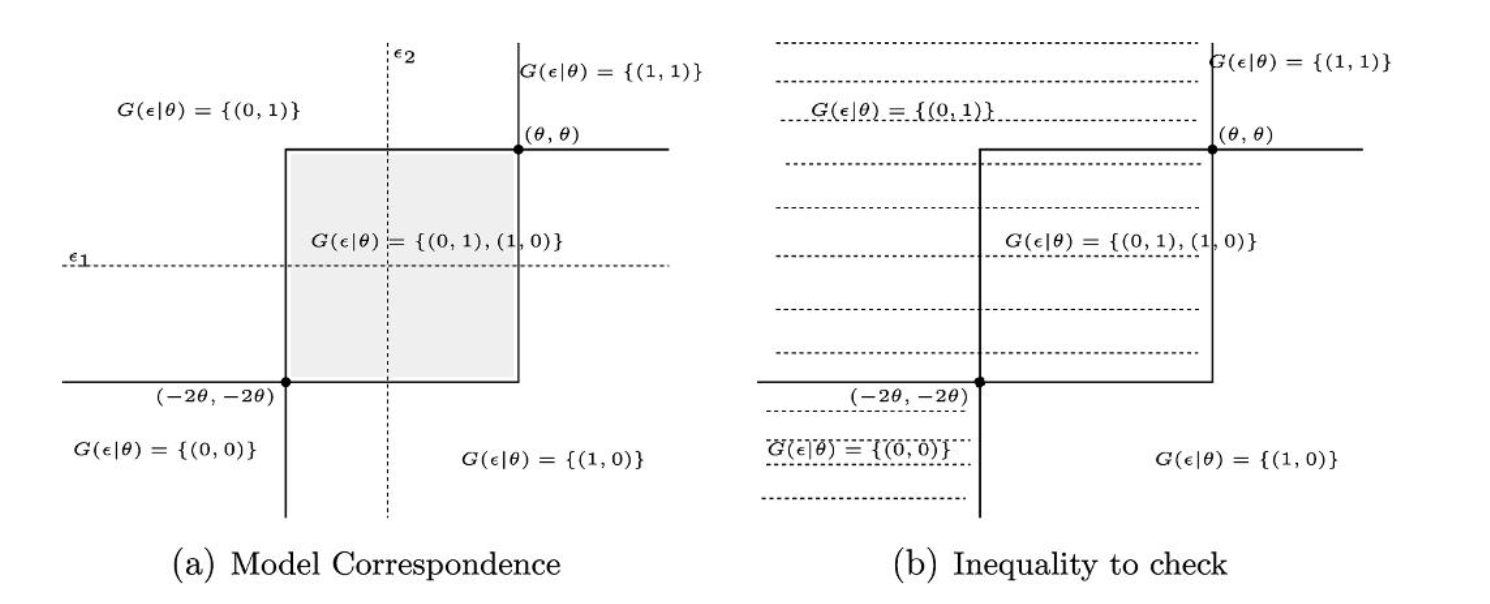
\includegraphics[width=0.95\textwidth]{figures/GH-Fig1}
	\caption{Family Game [Lifted from Paper]}
	\label{fig:GH-1}
\end{figure}

In the case of the family bargaining game, the set of possible outcomes is $\calY = \{(0,0),(0,1),(1,0),(1,1)\}$. The generalized likelihood of outcomes predicted by the model can be written as follows:
\begin{align*}
 	\calL(\{(0,0)\}|\theta) &= \nu(\eps: \eps_1 \leq -2\theta, \eps_2 \leq -2\theta| \theta) = \nu(G^{-1}((0,0)|\theta)|\theta)\\
 	\calL(\{(0,1)\}|\theta) &= \nu(\eps: \eps_1 \leq \theta, \eps_2 \geq -2\theta| \theta) = \nu(G^{-1}((0,1)|\theta)|\theta)\\
 	\calL(\{(1,0)\}|\theta) &= \nu(\eps: \eps_1 \geq -2\theta, \eps_2 \leq \theta| \theta) = \nu(G^{-1}((1,0)|\theta)|\theta)\\
 	\calL(\{(1,1)\}|\theta) &= \nu(\eps: \eps_1 \geq \theta, \eps_2 \geq \theta| \theta) = \nu(G^{-1}((1,1)|\theta)|\theta)
\end{align*}
anf the generalized likelihood of the remaining events can be derived as follows
\begin{align*}
	\calL(\{(0,0)\}\cup A | \theta) &= \calL(\{(0,0)\}|\theta) + \calL(A|\theta),\hbox{ }\text{ for all }A \subset \calY/\{(0,0)\}\\
	\calL(\{(1,1)\}\cup A | \theta) &= \calL(\{(1,1)\}|\theta) + \calL(A|\theta),\hbox{ }\text{ for all }A \subset \calY/\{(1,1)\} \\
	\calL(\{(0,1),(1,0)\}|\theta) &= 1 - \calL(\{(0,0),(1,1)\}|\theta)
\end{align*}
The generalized likelihood predicted by the model is the set function $A\mapsto \calL(A|\theta) = \nu(G^{-1}(A|\theta)|\theta)$ for $A \subset \calY = \{(0,0),(0,1),(1,0),(1,1)\}$. This set function is a Choquet capacity and if the support of $\nu$ is sufficiently large, the generalized likelihood sums to more than one because the region of multiple equilibria is ``counted twice''.

Model is completed by adding an equilibrium selection mechanism that will pick out a single equilibrium for each value of the latent variable $\epsilon$ in the region of multiplicity. As formally defined previously, an equilibrium selection mechanism is a conditional probability $\pi(\cdot | \eps, X,\theta)$ with support included in $G(\eps|X;\theta)$. It is compatible with the data if the probabilities it predicts are equal to the true probabilities of the observable variables.

In this example, for $j = 0,1$:
\[P((i,j)|X) = \int_\calU \pi((i,j)|\eps, X;\theta)\nu(d\eps|X;\theta)\]
Since the model contains no prior information, any valid probability measure equilibrium selection mechanism that generates equates predicted probabilities with observed probabilities is consistent.

It is noted that the definition of the identified region using a semi-parametric likelihood representation, with the equilibrium selection mechanism as the infinite dimensional nuisance parameter $\pi$ is impracticable, so Theorem \ref{thm:GH-1} is used to make it operational and compute $\Theta_I$. So
\[\Theta_I = \{\theta \in \Theta: (\forall A \in 2^\calY; P(A|X) \leq \calL(A|X;\theta); X-a.s\}\]

\subsection{Efficient Computation of the Identified Set}

Subtitle: ``\emph{Which inequalities to check and how to check them?}''

Describe three approaches to the effective computation of the identified set based on the characterization of Theorem~$\ref{thm:GH-1}$. First approach is based on submodular optimization and extends readily to the case with mixed strategies. Second approach, describes in Section 2.2, relies on the highly efficient algorithms for optimal transportation problems.\footnote{I found the following ArXiv introduction to optimal transport problems \href{https://arxiv.org/abs/1009.3856}{here} (if the link doesn't work; https://arxiv.org/abs/1009.3856)} Third approach is based off the notion of \emph{core determining sets} and provides a dramatic reduction in the computational complexity under specific assumptions on the game under study.

\subsubsection{Submodular Optimization}

The first proposal to deal with the complexity of the problem of checking inequalities in Theorem~\ref{thm:GH-1} is a method of general validity based on the minimization of a submodular function, the discrete equivalent of a convex function. This is a well-known problem in combinatorial optimization and efficient algorithms are easily available off the shelf.

\begin{definition}[Submodular function]
	\label{def:GH-6}
	A set function $\calL:\calY\rightarrow\SR$ is called submodular if, for each $A, B \subset \calY$, we have
	\[\calL(A\cup B) + \calL(A\cap B) \leq \calL(A) + \calL(B)\]
	In the case that $\calL$ is a probability measure, this holds as equality.
\end{definition}

Submodularity for set functions is the analogue of convexity, and the problem of minimizing a submodular function is well studied. Paper now shows that checking inequalities involved in the characterization of the identified set in Theorem~\ref{thm:GH-1} is equivalent to the minimization of a submodular function. Theorem~\ref{thm:GH-1} whose that the identified set is the set of values of $\theta$ such that $X$-almost surely, we have the domination $\forall A\subseteq \calY$, $P(A|X) \leq \calL(A|X;\theta)$. Equivalently,
\[\min_{A\subseteq\calY}\left(\calL(A|X;\theta) - P(A|X) \right) \geq 0\]
First note that the function above is indeed submodular.
\begin{lemma}[Submodularity of the generalized likelihood]
 	\label{lemma:GH-1}
	For all $\theta \in \Theta$ and all $X$, the set function $\calY$ defined for all $A\subseteq\calY$ by $A\mapsto \calL(A|X;\theta) - P(A|X)$ is submodular.
\end{lemma}
 The most efficient, generic, way to check that a convex function is everywhere non-negative and verify that the minimum is non-negative. Apply the same logic to the above. Of course, can speed this up by terminating the algorithm when a negative value is found.

 \begin{theorem}[Computation of the identified set]
	\label{thm:GH-2}
	The identified set is obtained by minimization of a submodular function
	\[\theta_I = \left\{\theta \in \Theta: \min_{B\subseteq\calY} \left(\calL(B|X;\theta - P(B|X)\right)= 0, X-\text{a.s}\right\}\]
 \end{theorem}

As a note: I think the reason there is an ``$=0$'' instead of a $\geq 0$ in the statement of the identified set above is that we can always take $B=\emptyset$. More details on the procedure are given later on in Section 4. This method can be generalized to the case where equilibria in mixed strategies are considered.

The below is a special case of submodular optimization which is more efficient and applies to the case where only equilibria in pure strategies are considered.

\subsubsection{Optimal Transportation Approach}

When equilibria are only in pure strategies, the model generalized likelihood $\calL$ is a very special case of submodular function since it is derived as the distribution function of a random set.
\[\calL(A|X;\theta) = \nu(\epsilon: G(\epsilon | X;\theta) \cap A \neq \emptyset| X;\theta)\]

When mixed equilibria are considered, this improvement in efficiency is no longer available because (in general), the model generalized likelihood is no longer the distribution of a random set.\footnote{Why not? I think because the probabilities of observing an outcome now are not functions of the underlying probability space $(\Omega, \calF, \mathbb{P})$, but, rather also depend on the properties of the mixed strategy equilibrium} To describe the method, need the following notations and definitions.

Call $\calU^*$ the set of predicted combinations of equilibrium, formally $\calU^* = \{G(\epsilon|X;\theta); \epsilon \in \calU\}$, remembering that $\calU$ is the support of $\eps$. Note that $\calU^*$ is a quotient space for the correspondence $G$
\footnote{From WolframMathWorld: A quotient space, $X$/{\raise.17ex\hbox{$\scriptstyle\mathtt{\sim}$}} of a topological space $X$ and a set of equivalence classes {\raise.17ex\hbox{$\scriptstyle\mathtt{\sim}$}} on $X$ is the set of equivalence classes of points in $X$ (under {\raise.17ex\hbox{$\scriptstyle\mathtt{\sim}$}}). Open sets on $X$/{\raise.17ex\hbox{$\scriptstyle\mathtt{\sim}$}} can be described using the map $\pi: X\rightarrow X$/{\raise.17ex\hbox{$\scriptstyle\mathtt{\sim}$}} which maps each point in $X$ to its equivalence class. A subset $W \subseteq X$/{\raise.17ex\hbox{$\scriptstyle\mathtt{\sim}$}} is open if $\pi^{-1}(W)$ is open. $\calU^*$ is a quotient space for $\calU$ using equivalence classes from the correspondence $G$, that is $\calU = X/${\raise.17ex\hbox{$\scriptstyle\mathtt{\overset{G}\sim}$}} where $\eps_1{\raise.17ex\hbox{$\scriptstyle\mathtt{\overset{G}\sim}$}} \eps_2$ if $G(\eps_1) = G(\eps_2)$}.
So $\calU^*$ contains subsets of $\calY$ but is typically of much lower cardinality than $2^\calY$.

Further, consider the bipartite graph $\calG(\theta, X)$ in $\calY \times \calU^*$. The edges are defined as $(y,u) \in E(\calG)$ if $y \in u$. Each vertex $u \in \calY$ has weight $P(y|X)$ and each vertex $y\in \calU^*$ has weight $\nu(\{\epsilon: G(\epsilon|X;\theta) = u|X\})$. Finally, call $Q(\cdot|X;\theta)$ the probabilities $Q(u|X;\theta) = \nu\{G^{-1}(u)| X;\theta)\}$ (so t at $Q(u|X;\theta)$ is the weight attached to vertex $u \in \calY$.)

To summarize:

\begin{enumerate}
	\item \(\calY\) is the set of all possible (observed) outcomes
	\item \(G(\eps | X;\theta)\) is the (measurable) {\it equilibrium correspondence} from the underlying probability space onto \(\calY\). For any open subset \(A \subset \calY\),
	\[G^{-1}(A|X;\theta) := \{\eps\in\calU: G(\eps|X;\theta) \cap A \neq \emptyset\}\]
	is measurable
	\item \(\eps\) is distributed according to the probability measure $\nu(\cdot | X;\theta)$ on \(\calU\)
	\item The model generalized likelihood, \(\calL: 2^\calY \to [0,1]\) is given
	\[\calL(A|X;\theta) := \nu(G^{-1}(A | X;\theta) | X;\theta)\]
	\item \(\calU^*\) is the set of all predicted combinations of equilibria. That is \(\calU^* = \{G(\eps|X;\theta): \eps \in \calU\} \subset 2^\calY\)
	\item Optimal Transportation approach is considering a bipartite graph \(\calG(X;\theta)\) on $\calY \times \calU^*$
	\begin{enumerate}
		\item Edges link $y \in \calY$ to $u\in \calU^*$ if $y \in u$. So $(y,u) \in E(\calG(X;\theta))$ if $y \in u$.
		\item \(Q(\cdot|X;\theta)\) is a probability distribution over $2^\calY$ with support $\calU^*$ induced by the equilibrium correspondence.
		\[Q(u|X;\theta) = \nu(\{\eps: G(\eps|X;\theta) = u | X;\theta\})\]
		\item Vertex $y\in \calY$ has weight $P(y|X)$ and each vertex $u\in \calU^*$ has weight $Q(u|X;\theta)$
	\end{enumerate}
\end{enumerate}

Theorem~\ref{thm:GH-1} shows that $\theta \in \Theta_I$ if and only if, for any subset $A$ of $\calY$, we have $P(A|X) \leq Q(G^{-1}(A)|X;\theta)$, where $G^{-1}(A) = \{u\in\calU^* | A\cap u \neq \theta\}$. Galichon and Genry show that it is equivalent to the existance of a joint probability $\Lambda$ on $\calG(\theta, X)$ with marginal distributions $P(\cdot| X)$ and $Q(\cdot|X;\theta)$.\footnote{I'm a bit lost on this part. I don't quite know what a probability is on a bipartite graph. I guess we just mean a joint probability distribution on the product space of the outcomes and the sets of outcomes. The theorem makes more sense intuitively looking at it from this view. For a consistent parameter, the rules relating the weights on one side with weights on the other are given above.}

\begin{theorem}
	\label{thm:GH-3}
	The parameter value $\theta$ belongs to the identified set iff there exists a probability on $\calY \times \calU^*$ with support contained in $G(X;\theta)$ and with marginal probabilities $P(\cdot|X)$ and $Q(\cdot|X;\theta)$.
\end{theorem}

One implication is easy to prove. Call $U$ the random element with distribution $Q$ ($U$ is the ``preimage'' of $Q(u|X;\theta)$ from $(\Omega, \calF, \mathbb{P}) \rightarrow 2^\calY$) If a joint probability $\Lambda$ exists with all the required properties then
\[Y\in A \implies U\in G^{-1}(A)\footnote{How I think about this: $Y$ is a map from $\epsilon$ onto $\calY$. \(U\) maps from $\epsilon$ to $\calU^*$. $Y$ gives the observed equilibria, $U$ gives all the possible outcomes. $A$ is a set of possible outcomes. The observed outcome must be a possible outcome. So if the observed outcome is in $A$, then t he set of possible outcomes must also intersect $A$. So $Y\in A\rightarrow U \in G^{-1}(A)$}\]
so that $\ind_{\{Y\in A\}} \leq \ind_{\{U\in G^{-1}(A)\}}$, \(\Lambda\)-a.s. Taking expectations, gives \(\E_\Lambda(\ind_{\{Y\in A\}}) \leq \E_\Lambda(\ind_{\{ U\in G^{-1}(A) })\). Equivalently, $\P(A|X) \leq Q(G^{-1}(A)|X;\theta)$. The converse is more involved and relies on optimal transportation theory. A similar result is proved in Theorem 3 of Artstein (1983), based on an extension of the marriage lemma.


\begin{example*}[Family Bargaining Example cont.] For the case of the family bargaining game
\[\calU^* = \bigg\{\{(0,0)\}, \{(0,1)\}, \{(1,0)\}, \{(1,1)\}, \{(0,1),(1,0)\}\bigg\}\]
The bipartite graph depicting this is in Figure \ref{fig:GH-Fig2}(a), where $p_y, y \in \calY$ denotes $\P(y|X)$ and $q_u, y\in \calU^*$ denotes $\nu(\{\eps: G(\eps|X;\theta) = u | X;\theta\})$. The existence of a joint probability on $\calY \times \calU^*$ supported on $\calG(X;\theta)$ with marginal probabilities $p_y, y\in \calY$ and $q_u, u\in \calU^*$ can be represented graphically by a set of non-negative numbers attached to each edge of the graph that sum to 1 and such that the weight of each vertex is equal to the sum of the weights on the edges that reach it. For instance, a joint probability is denoted $\alpha_y^u$ for $(y,u)\in \calY\times\calU^*$ and must satisfy $\alpha_y^u \geq 0$ for all $(y,u)\in \calY\times\calU^*$, $\alpha_y^u = 0$ if $y\not\in u$, $\sum_{y\in u} \alpha_y^u = 1$ and equalities such as $p_{01} = \alpha_{01}^{01} + \alpha_{01}^{01,10}$ and $q_{01,10} = \alpha_{01}^{01,10} + \alpha_{10}^{01,10}$.

\begin{figure}[htb!]
	\centering
	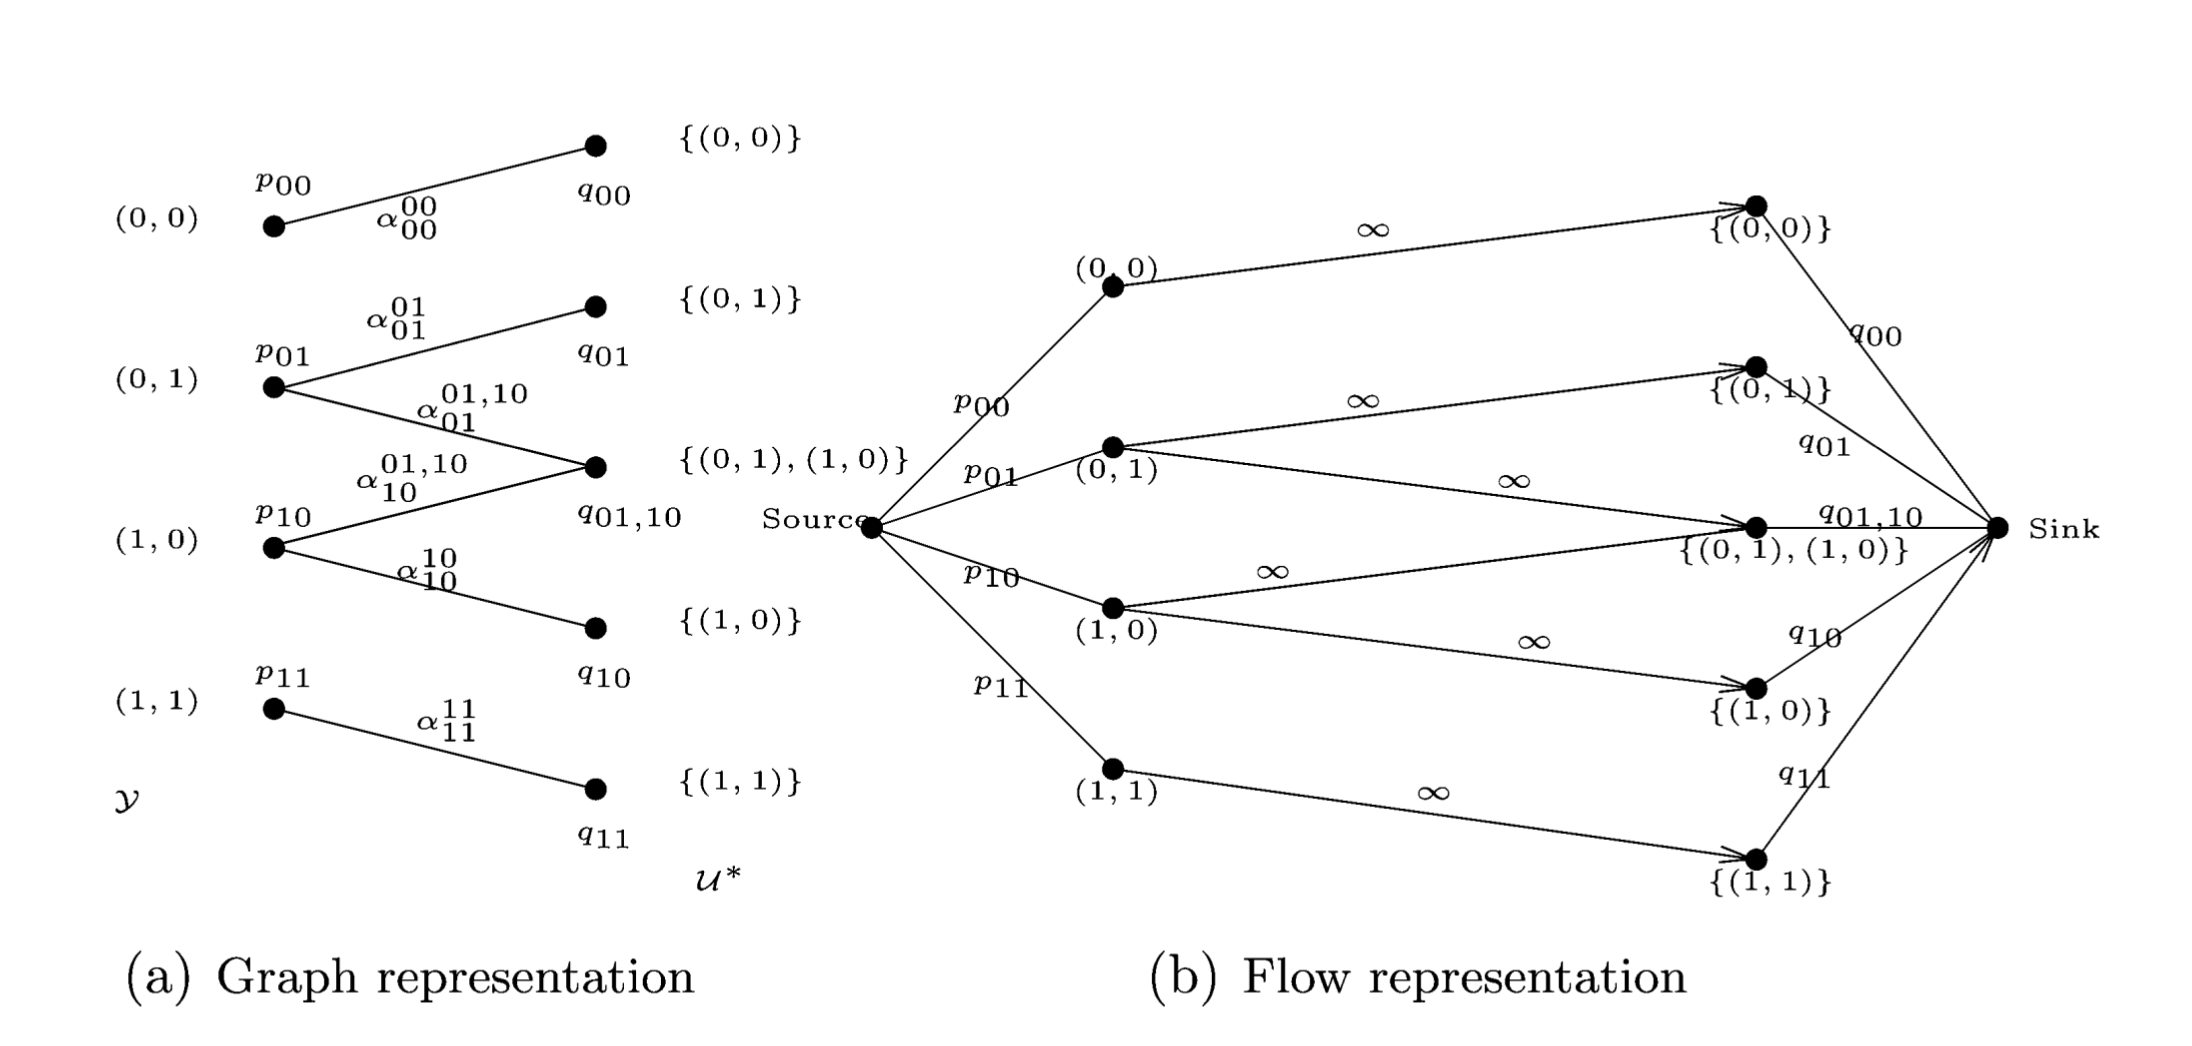
\includegraphics[width=0.95\textwidth]{figures/GH-Fig2.png}
	\caption{Family Game (continued), lifted from \citet{GH-2011}}
	\label{fig:GH-Fig2}
\end{figure}

\end{example*}
 
Since the problem of computing the identified set has now been formulated as on involving the existence of a probability measure with given marginal distributions, one can appeal to efficient computational methods in the optimal transportation literature. The problem of sending $p_y, y\in \calY$ \emph{units of a good} to $q_i, u\in\calU^*$ \emph{units in terminals}, $u\in \calU^*$ at minimum cost of transportation, where costs are attached to each pair $(y,u) \in \calY\times\calU^*$ is called an optimal transportation problem
\footnote{Basically, we have a total of 1 unit of ``good'' on the left hand ($\calY$) side, split over the elements of $\calY$ and 1 unit of ``capacity'' on the right hand side ($\calU^*$) split over the units of $\calU^*$. We need to get the goods on the left hand side to the right hand side, but can only use the paths $(y,u)\in\calG(X;\theta)$). Because there is one unit of good on the LHS and 1 total unit of capacity on the RHS, all carrying units on the RHS are ``filled''. This is equivalent to there being a valid equilibrium selection mechanism.}. The problem at hand can be reduced to an optimal transportation problem where a pair $(y,u)$ is assigned cost zero if it belongs to $\calG(X;\theta)$ and one otherwise. There exists a joint law on $\calG(x;\theta)$ with marginals $P$ and $Q$ (that is $\theta\in\Theta_I$) if and only if there is a zero-cost solution to the optimization problem thus defined. This minimum cost of transportation problem has an equivalent dual formulation as a maximum flow problem described in Figure \ref{fig:GH-Fig2}(b). The edges in the graph with 0 cost in th minimum cost of transportation problem have infinite carrying capacity in the dual maximum flow problem. So, efficient maximum flow programs can be applied directly to the network described in Figure 2(b): mass flows from the source to the sink through the network. 

\subsubsection{Core-determining classes}

Theorem \ref{thm:GH-1} allows reduction of the problem of computing the identified set to that of checking a set of inequalities. However, the computational burden is only partially lifted, as the number of inequalities to check can be very large if the cardinality of the outcomes space is large. This section will analyze ways of reducing this remaining computational burden by eliminating redundant inequalities in the computation of the identified set. This is formalized with the concept of \emph{core determining classes}, first introduced in \citet{GH-2006}.

\begin{definition}[Core Determining]
	\label{def:GH-7}
	A class $\calA$ of measurable subsets of $\calY$ is called \emph{core determining} for the Choquet capacity $\calL$ on $\calY$ if it sufficient to characterize the core of $\calL$, i.e if a probability $Q \in \text{core}(\calL)$ when $Q(A) \leq \calL(A)$ for all $A\in\calA$.
\end{definition}

A core-determining class of sets is sufficient to characterize the identified region $\Theta_I$ as summarized in the following proposition:
\begin{prop}
	\label{prop:GH-1}
	If $\calA$ is core determining for the Choquet capacity $A\mapsto\calL(A|X;\theta) = \nu(\eps:G(\eps|X;\theta)\cap A \neq \emptyset | X;\theta)$, $X$-a.s, and for all $\theta$, then
	\begin{align*}
	 	\Theta_I = \{\theta\in \Theta: \forall A\in\calA, P(A|X) \leq \calL(A|X), X\text{-a.s}\}
	 \end{align*} 
\end{prop}
Challenge therefore becomes that of finding a core-determining class $\calA$ in order to reduce the number of inequalities to be checked to the cardinality of $\calA$. Return to the family bargaining example to illustrate:
\begin{example*}[Family Bargaining cont.]
	Return to the family bargaining game and consider some proposal for the computation of the identified set proposed in the literature. Call the \emph{Singleton class} the class of singleton sets $\{\{(0,0)\},\{(0,1)\},\{(1,0)\}, \{(1,1\}\}$. It is immediate to see that this class is not core determining in general. Indeed if $\eps$ has large enough support, the two equalities $\P(\{(0,1)\}) = \nu(G(\eps|\theta)\cap\{(0,1)\}\neq \emptyset|\theta) = \nu(\eps:\eps_1 \leq\theta, \eps_2 \geq -2\theta|\theta)$ and $P(\{(1,0\}) = \nu(G(\eps|\theta)\cap\{(1,0)\}\neq \emptyset|\theta)$ jointly imply $\P(\{(0,1),(1,0)\}) > \nu(G(\eps|\theta)\cap\{(0,1),(1,0)\}\neq \emptyset|\theta)$
\end{example*}

Now show how to identify core-determining classes more generally to avoid case-by-case elimination of redundant inequalities. To this end, give general conditions under which one can find a core-determining class of low cardinality. Recall a subset $A$ of an ordered set (equipped with $\succsim$) is said to be \emph{connected} if any $a$ such that $\sup A \succsim a \succsim \inf A$ belongs to $A$\footnote{For example $[0,1]$ is connected while $(0,1)$ and $[0,1] \cup [2,3]$ are not}.

\begin{assumption}[Monotonicity]
	\label{assm:GH-2}
	There exists an ordering $\succsim_\calY$ of the set of outcomes $\calY$ and an ordering $\succsim_\calU$ of the set of latent variables $\calU$ such that $G(\eps|X;\theta)$ is connected for all $\eps\in\calU$, $X$-a.s, all $\theta$, and $\sup G(\eps_2|X;\theta) \succsim_\calY\sup G(\eps_1|X;\theta)$ and $\inf G(\eps_2|X;\theta) \succsim_\calY \inf G(\eps_1|X;\theta)$ when $\eps_2\succsim_\calU \eps_1$. Both orderings are allowed to depend on the exogenous variables $X$,but the dependence is suppressed in the notation for clarity.\footnote{ This assumption is related to monotone comparative statics in supermodular games}
\end{assumption}
\begin{example*}[Family bargaining cont.]
	IN the family bargaining game, the orderings are very simple to construct. A lexicographic order on $\calY$ is suitable with $(0,0)\precsim_\calY (0,1)\precsim_{\calY} (1,0) \precsim_{\calY})(1,1)$. On $\calU$ the ordering is related to predicted outcomes. All $\eps$ producing the same predicted outcomes will be equivalent, and the ordering on predicted outcomes is $\{(0,0)\}\precsim_\calU \{(0,1)\} \precsim_\calU \{(0,1),(1,0)\}\precsim_\calU \{(1,0)\}\precsim_\calU \{(0,1)\}$. Here $A_1 \precsim_\calU A_2$ is a short-hand notation for $\eps_1 \precsim_\calU \eps_2$ if $G(\eps_1|X;\theta) = A_1$ and $G(\eps_2 | x;\theta) = A_2$.

	For instance, taking $\eps_1$ such that $G(\eps_1 | X;\theta) = \{(0,1)\}$ and $\eps_2$ such that $G(\eps_2|\theta) = \{(0,1),(1,0)\}$ we have $\sup G(\eps_1|\theta) = (0,1) \precsim_{\calY} (1,0) = \sup G(\eps_2 | \theta)$ and $\inf G(\eps_1 | \theta) = (0,1) = \inf G(\eps_2 |\theta)$\footnote{Here it is useful to remember that the infima and suprema are being taken with respect to the orderings $\succsim_\calU$ and $\succsim_\calY$.} This is illustrated in Figure \ref{fig:GH-Fig3}.
\end{example*}

\begin{figure}[htb!]
	\centering
	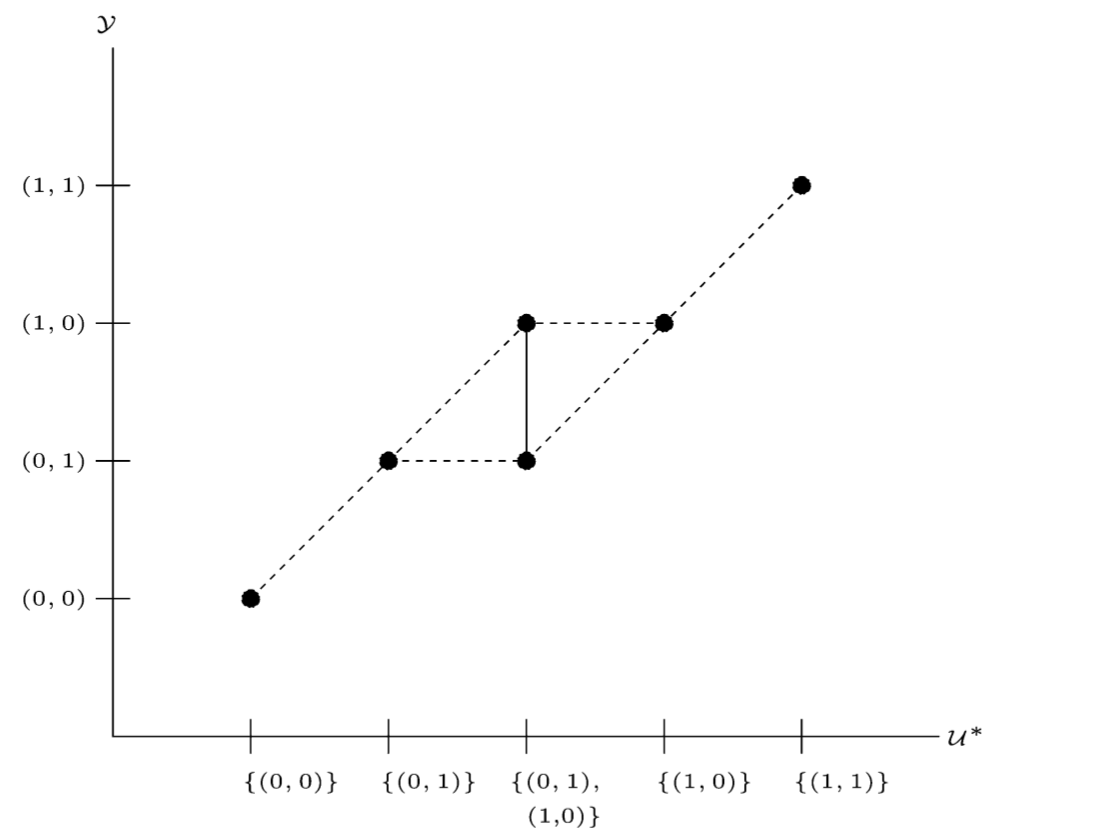
\includegraphics[width=0.75\textwidth]{figures/GH-Fig3.png}
	\caption{The monotonicity assumption in Assumption 2 is satisfied for this choice of orderings in the family bargaining example. The thick dots represent the correspondence $G(\cdot | \theta)$, $\calU^*$ denotes the ordered set of combinations of equilibria.}
	\label{fig:GH-Fig3}
\end{figure}
This sets up the theorem, which is the main tool in the construction of core-determining classes, and hence in the compuation of the identified set under the monotonicity assumption.
\begin{theorem}
	\label{thm:GH-4}
	Suppose Assumption \ref{assm:GH-2} is satisfied with orderings $\succsim_\calY$ and $\succsim_\calU$. Cal $I$ the cardinality of $\calY$ and list outcomes (elements of $\calY$) in increasing order (w.r.t $\succsim_\calY$) as $y_1, \dots, y_I$. Then $\calA = (\{y_1, \dots, y_i\},\{y_i,\dots, y_I\}, i = 1,\dots, I)$ is core determining. 
\end{theorem}

Theorem \ref{thm:GH-4} allows to reduce the cardinality of the power set $2^\calY$ to twice the cardinality of $\calY$ minus $2$, since the inequality need not be checked on the whole set $\calY$. 

\subsection{Illustration: Oligopoly Entry with Two Types of Players}

Now turn to a more substantive illustration of methods to compute the identified set. First, to show the operational usefulness of Theorem \ref{thm:GH-4}. To do so, consider the oligopoly entry game with two types of players presented in Appendix $A$ of Berry and Tamer (2006). 

The profit function of of Type 1 firms depends on the total number of firms in the market, but not on the type of those firms, while the profits of Type 2 firms depend both on the number and on the type of firms present in the market. The latent variable is the fixed cost $f_1$ for firms of Type 1 and $f_2$ for firms of type 2. Assume \((f_1, f_2) \sim \text{Unif}([0,1]^2)\). Model is simplified by assuming linearity of profits in the firm number as follows: 
\begin{align*}
	\Pi_1(Y_1, Y_2, X, f;\theta) &= \alpha_0 + \alpha_1(Y_1 + Y_2) + \alpha_2 X - f_1 \\ 
	\Pi_2(Y_1, Y_2, X, f;\theta) &= \beta_0 + \beta_1 + \beta_2 Y_2 + \beta_3 X - f_2
\end{align*}
with $\alpha_1, \beta_1, \beta_2 < 0$ and $\beta_1 > \beta_1$. Set of observable outcomes is


